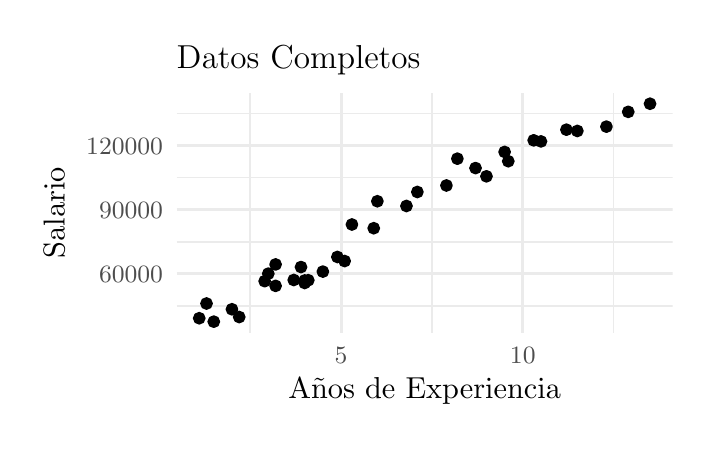
\begin{tikzpicture}[x=1pt,y=-1pt,scale=1.00]
\fill[fill={rgb,255:red,255; green,255; blue,255}] (0,0) rectangle (238.52,142.22);
\begin{scope}\clip (0.00,0.00) rectangle (238.52,142.22);
\end{scope}\begin{scope}\clip (53.85,23.54) rectangle (233.04,110.17);
\draw[line width=0.53pt,draw={rgb,255:red,235; green,235; blue,235},line join=round] (53.85,100.61) -- (233.04,100.61);
\draw[line width=0.53pt,draw={rgb,255:red,235; green,235; blue,235},line join=round] (53.85,77.38) -- (233.04,77.38);
\draw[line width=0.53pt,draw={rgb,255:red,235; green,235; blue,235},line join=round] (53.85,54.16) -- (233.04,54.16);
\draw[line width=0.53pt,draw={rgb,255:red,235; green,235; blue,235},line join=round] (53.85,30.94) -- (233.04,30.94);
\draw[line width=0.53pt,draw={rgb,255:red,235; green,235; blue,235},line join=round] (80.38,110.17) -- (80.38,23.54);
\draw[line width=0.53pt,draw={rgb,255:red,235; green,235; blue,235},line join=round] (146.07,110.17) -- (146.07,23.54);
\draw[line width=0.53pt,draw={rgb,255:red,235; green,235; blue,235},line join=round] (211.76,110.17) -- (211.76,23.54);
\draw[line width=1.07pt,draw={rgb,255:red,235; green,235; blue,235},line join=round] (53.85,89.00) -- (233.04,89.00);
\draw[line width=1.07pt,draw={rgb,255:red,235; green,235; blue,235},line join=round] (53.85,65.77) -- (233.04,65.77);
\draw[line width=1.07pt,draw={rgb,255:red,235; green,235; blue,235},line join=round] (53.85,42.55) -- (233.04,42.55);
\draw[line width=1.07pt,draw={rgb,255:red,235; green,235; blue,235},line join=round] (113.23,110.17) -- (113.23,23.54);
\draw[line width=1.07pt,draw={rgb,255:red,235; green,235; blue,235},line join=round] (178.91,110.17) -- (178.91,23.54);
\draw[fill={rgb,255:red,0; green,0; blue,0},line width=0.71pt,line cap=round,line join=round] (61.99,104.99) circle (1.95);
\draw[fill={rgb,255:red,0; green,0; blue,0},line width=0.71pt,line cap=round,line join=round] (64.62,99.67) circle (1.95);
\draw[fill={rgb,255:red,0; green,0; blue,0},line width=0.71pt,line cap=round,line join=round] (67.25,106.23) circle (1.95);
\draw[fill={rgb,255:red,0; green,0; blue,0},line width=0.71pt,line cap=round,line join=round] (73.81,101.75) circle (1.95);
\draw[fill={rgb,255:red,0; green,0; blue,0},line width=0.71pt,line cap=round,line join=round] (76.44,104.56) circle (1.95);
\draw[fill={rgb,255:red,0; green,0; blue,0},line width=0.71pt,line cap=round,line join=round] (85.64,91.60) circle (1.95);
\draw[fill={rgb,255:red,0; green,0; blue,0},line width=0.71pt,line cap=round,line join=round] (86.95,88.88) circle (1.95);
\draw[fill={rgb,255:red,0; green,0; blue,0},line width=0.71pt,line cap=round,line join=round] (89.58,93.30) circle (1.95);
\draw[fill={rgb,255:red,0; green,0; blue,0},line width=0.71pt,line cap=round,line join=round] (89.58,85.55) circle (1.95);
\draw[fill={rgb,255:red,0; green,0; blue,0},line width=0.71pt,line cap=round,line join=round] (96.15,91.17) circle (1.95);
\draw[fill={rgb,255:red,0; green,0; blue,0},line width=0.71pt,line cap=round,line join=round] (98.77,86.50) circle (1.95);
\draw[fill={rgb,255:red,0; green,0; blue,0},line width=0.71pt,line cap=round,line join=round] (100.09,92.25) circle (1.95);
\draw[fill={rgb,255:red,0; green,0; blue,0},line width=0.71pt,line cap=round,line join=round] (100.09,91.35) circle (1.95);
\draw[fill={rgb,255:red,0; green,0; blue,0},line width=0.71pt,line cap=round,line join=round] (101.40,91.26) circle (1.95);
\draw[fill={rgb,255:red,0; green,0; blue,0},line width=0.71pt,line cap=round,line join=round] (106.66,88.14) circle (1.95);
\draw[fill={rgb,255:red,0; green,0; blue,0},line width=0.71pt,line cap=round,line join=round] (111.91,82.85) circle (1.95);
\draw[fill={rgb,255:red,0; green,0; blue,0},line width=0.71pt,line cap=round,line join=round] (114.54,84.33) circle (1.95);
\draw[fill={rgb,255:red,0; green,0; blue,0},line width=0.71pt,line cap=round,line join=round] (117.17,71.12) circle (1.95);
\draw[fill={rgb,255:red,0; green,0; blue,0},line width=0.71pt,line cap=round,line join=round] (125.05,72.46) circle (1.95);
\draw[fill={rgb,255:red,0; green,0; blue,0},line width=0.71pt,line cap=round,line join=round] (126.36,62.72) circle (1.95);
\draw[fill={rgb,255:red,0; green,0; blue,0},line width=0.71pt,line cap=round,line join=round] (136.87,64.43) circle (1.95);
\draw[fill={rgb,255:red,0; green,0; blue,0},line width=0.71pt,line cap=round,line join=round] (140.81,59.37) circle (1.95);
\draw[fill={rgb,255:red,0; green,0; blue,0},line width=0.71pt,line cap=round,line join=round] (151.32,57.02) circle (1.95);
\draw[fill={rgb,255:red,0; green,0; blue,0},line width=0.71pt,line cap=round,line join=round] (155.27,47.34) circle (1.95);
\draw[fill={rgb,255:red,0; green,0; blue,0},line width=0.71pt,line cap=round,line join=round] (161.83,50.73) circle (1.95);
\draw[fill={rgb,255:red,0; green,0; blue,0},line width=0.71pt,line cap=round,line join=round] (165.78,53.71) circle (1.95);
\draw[fill={rgb,255:red,0; green,0; blue,0},line width=0.71pt,line cap=round,line join=round] (172.34,44.90) circle (1.95);
\draw[fill={rgb,255:red,0; green,0; blue,0},line width=0.71pt,line cap=round,line join=round] (173.66,48.25) circle (1.95);
\draw[fill={rgb,255:red,0; green,0; blue,0},line width=0.71pt,line cap=round,line join=round] (182.85,40.70) circle (1.95);
\draw[fill={rgb,255:red,0; green,0; blue,0},line width=0.71pt,line cap=round,line join=round] (185.48,41.10) circle (1.95);
\draw[fill={rgb,255:red,0; green,0; blue,0},line width=0.71pt,line cap=round,line join=round] (194.68,36.86) circle (1.95);
\draw[fill={rgb,255:red,0; green,0; blue,0},line width=0.71pt,line cap=round,line join=round] (198.62,37.32) circle (1.95);
\draw[fill={rgb,255:red,0; green,0; blue,0},line width=0.71pt,line cap=round,line join=round] (209.13,35.76) circle (1.95);
\draw[fill={rgb,255:red,0; green,0; blue,0},line width=0.71pt,line cap=round,line join=round] (217.01,30.42) circle (1.95);
\draw[fill={rgb,255:red,0; green,0; blue,0},line width=0.71pt,line cap=round,line join=round] (224.89,27.48) circle (1.95);
\end{scope}\begin{scope}\clip (0.00,0.00) rectangle (238.52,142.22);
\node[text={rgb,255:red,77; green,77; blue,77},anchor=base east,inner sep=0pt, outer sep=0pt, scale=1.00] at (48.91,92.14) {\fontsize{8.80}{\baselineskip}\selectfont 60000};
\node[text={rgb,255:red,77; green,77; blue,77},anchor=base east,inner sep=0pt, outer sep=0pt, scale=1.00] at (48.91,68.92) {\fontsize{8.80}{\baselineskip}\selectfont 90000};
\node[text={rgb,255:red,77; green,77; blue,77},anchor=base east,inner sep=0pt, outer sep=0pt, scale=1.00] at (48.91,45.69) {\fontsize{8.80}{\baselineskip}\selectfont 120000};
\node[text={rgb,255:red,77; green,77; blue,77},anchor=base,inner sep=0pt, outer sep=0pt, scale=1.00] at (113.23,121.39) {\fontsize{8.80}{\baselineskip}\selectfont 5};
\node[text={rgb,255:red,77; green,77; blue,77},anchor=base,inner sep=0pt, outer sep=0pt, scale=1.00] at (178.91,121.39) {\fontsize{8.80}{\baselineskip}\selectfont 10};
\node[text={rgb,255:red,0; green,0; blue,0},anchor=base,inner sep=0pt, outer sep=0pt, scale=1.00] at (143.44,134.10) {\fontsize{11.00}{\baselineskip}\selectfont Años de Experiencia};
\node[text={rgb,255:red,0; green,0; blue,0},rotate=90.00,anchor=base,inner sep=0pt, outer sep=0pt, scale=1.00] at (13.33,66.86) {\fontsize{11.00}{\baselineskip}\selectfont Salario};
\node[text={rgb,255:red,0; green,0; blue,0},anchor=base west,inner sep=0pt, outer sep=0pt, scale=1.00] at (53.85,14.90) {\fontsize{13.20}{\baselineskip}\selectfont Datos Completos};
\end{scope}
\end{tikzpicture}